\section{Privacy Profile}

\begin{frame}[red]
\frametitle{Privacy Profile}
\begin{itemize}
\item Settings
\item PSR - Potentially Sensitive Region
\item Protection types and schemes
\item t-anonymity
\end{itemize}
\end{frame}

\subsection{Settings} % Bookmark information, displayed in the progress tree

\begin{frame}[red] %hmm.. thought i could change colour here :S
\frametitle{Settings}

Users Can
\begin{itemize}
	\item Set both globally and locally
	\begin{itemize}
		\item Temporal sensitivity
		\item Spatial sensitivity
	\end{itemize}
	\item Define a PSR
	\item Have multiple profiles.
\end{itemize}

\vspace{1em}
\begin{definition}[Privacy Profile]
$\left(stime,etime,d_s, d_t,\{PSR \} \right)$
\end{definition}

\end{frame}



\begin{frame}[red] %hmm.. thought i could change colour here :S
\frametitle{PSR}
\begin{itemize}
\item A group of edges in a road network considered sensitive
\item A value indicating spatial sensitivity
\item A value indicating temporal sensitivity
\item A general usage class
\end{itemize}
\begin{definition}[PSR]
A PSR $p$ is a tuple $(p_{edges}, d_s, d_t, class)$ where $p_{edges}$ is the set of tuples $\{(e, e_{from}, e_{to} | 0 \leq e_{from} < e_{to} \leq e_{length})\}$ which is sensitive. 
$e \in \mathbf{E}$ and $e_{from}, e_{to}, e_{length} \in \mathbb{R}$. 
$e_{from}/e_{to}$ specifies on $e$ the start-/end-location covered by $p_{cover}$. If $e$ is fully included in $p_{cover}$, $e_{from}/e_{to}$ is equal to $0/p_{length}$.
$d_s, d_t, class \in \mathbb{N}$ is respectively the spatial sensitivity, the temporal sensitivity, and the PSR classification
\end{definition}
\end{frame}

\begin{frame}[red] %hmm.. thought i could change colour here :S
\frametitle{PSR Classes}

\begin{table}
%\begin{tabular*}{0.8\columnwidth}{|p{0.2\columnwidth}|l|p{0.25\columnwidth}|}
\begin{tabular}{|l|l|}
\hline
\bf Classification	& \bf Scheme \\\hline		
Public Service Point	& AS \\\hline
House			& ASTI,RS \\\hline
Route w. endpoints	& AS, ASTI, RS  \\\hline
Route w/o endpoints	& AS, ASTI, RS  \\\hline
\end{tabular}
\end{table}
\vspace{1em}

Protection Schemes
\begin{itemize}
	\item AS - Always Sensitive.
	\item ASTI - Always Sensitive within a time interval.
	\item RS - Rarely Sensitive.
\end{itemize}
\end{frame}


\subsection{t-anonymity} 
\begin{frame}[red]
\frametitle{t-anonymity}

Spatial k-anonymity 
\begin{itemize}
\item Adapted for trajectories
\item Argumented with time.
\end{itemize}
\vspace{1em}

In a PSR:
\begin{itemize}
\item Spatial sensitivity decides t-1 trajectories to hide between
% \vspace{1em}
\item Temporal sensitivity defines a time period shared with t-1 other trajectories.
\end{itemize}
\end{frame}


\begin{frame}[red] %hmm.. thought i could change colour here :S
\frametitle{Definition: t-anonymity}
\begin{definition}[t-anonymity]
Given $\mathbf{T}$, the set of trajectories and $p_{edges}$, the set of edges covering a sensitive part of trajectory $\gamma$. 

Let $\Gamma \subseteq \mathbf{T}$ be all trajectories which subtrajectories intersect with $p_{edges}$. $\Gamma' \subseteq \Gamma$ be all trajectories where, for edges intersecting with $p_{edges}$, at each timestamp of $\gamma$ their timestamps lie within a time period $TP$ symmetric around the timestamp of $\gamma$.

$\Gamma'$ is said to satisfy t-anonymity with respect to $TP$ and $\gamma$ iff $\Gamma'$ contains at least $t-1$ other trajectories.
\end{definition}
\end{frame}

\subsection{Time Period}
\begin{frame}[red]
\frametitle{Time Period}
\begin{columns}
	\begin{column}{0.5\textwidth}
		\only<1>{ 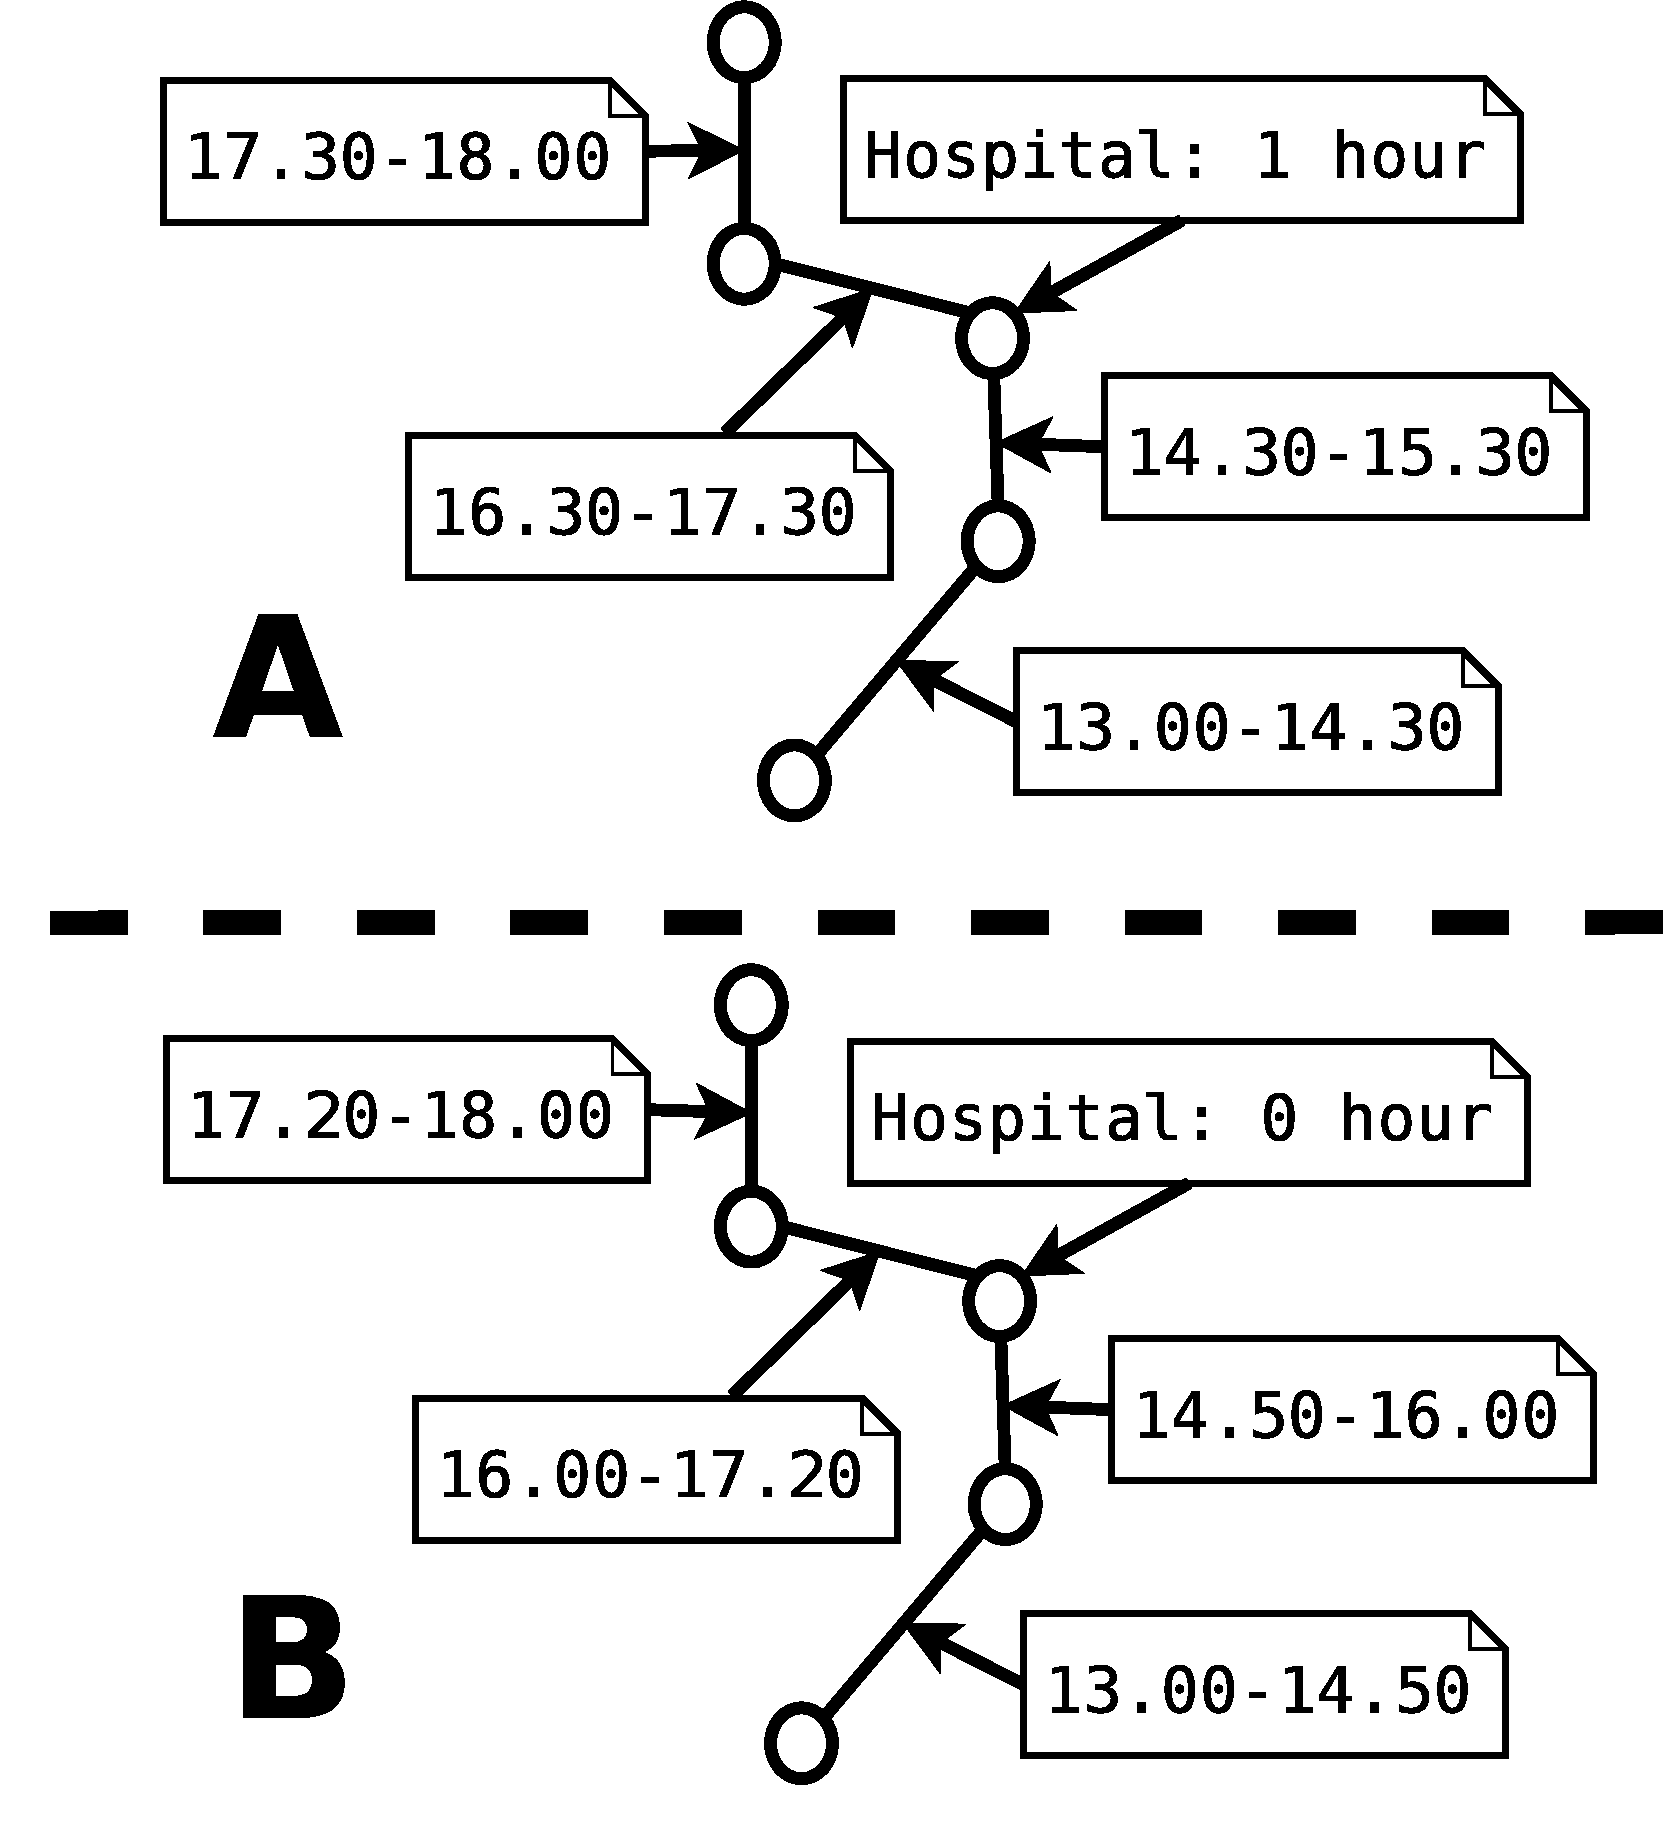
\includegraphics[scale=0.16]{images/trajecAdjustTime.pdf}}
	\end{column}
	\begin{column}{0.5\textwidth}
		\only<1>{ 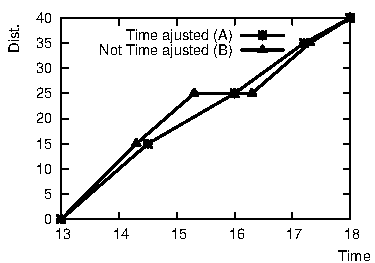
\includegraphics[scale=0.8]{images/trajecAdjustTimeGraph.pdf}}
	\end{column}
\end{columns}
\end{frame}